% !TeX root = ../main.tex
\documentclass[../main.tex, class=article, 12pt]{subfiles}
\usepackage{float}
\usepackage{amsthm}
\usepackage{amsmath}
\usepackage{amssymb}
\usepackage{hyperref}
\usepackage{caption}
\usepackage{mathtools}
\usepackage{graphicx}
\usepackage{todonotes}
\usepackage{tcolorbox}
\graphicspath{{./images}}




\begin{document}

\begin{align*}
        e = 1  +\frac{1}{1!} +\frac{1}{2!} +\frac{1}{3!}+\frac{1}{4!}+\ldots \\
\end{align*}

\begin{theorem}
       Se $ f(x) $ è una funzione crescente allora:
       \begin{equation*}
               \exists \lim_{x \to +\infty}f(x)= \begin{cases}+\infty \\ l \in \mathbb{R}\end{cases}
       \end{equation*}
       Se in particolare $ f(x) $ è \textbf{limitataa} allora:
       \begin{equation*}
               \exists \lim_{x \to 0} f(x) 
       \end{equation*}
       ed è un numero finito.
\end{theorem}
%\begin{corollario}
%       Stesso teorema per $ f $ decrescente (si consideri $ g = -f $)
%\end{corollario}


\subsection{Binomio di Newton}\label{sec:binomio_di_newton}
\begin{definition}
        Il binomio di Newton risponde alla domanda:
        \begin{equation*}
                {(x + y)}^n = ?  
        \end{equation*}
        Che sarebbe:
        \begin{align*}
                & {(x+1)}^1 = x + y \\
                & {(x+y)}^2 = x^2 + 2xy + y^2 \\
                & {(x+y)}^3 = {(x+y)}^2 * (x + y) = x^3 + 3x^2y+3xy^2+y^3 
        \end{align*}
\end{definition}

Possiamo notare un certo pattern nel risultato delle varie equazioni, questo pattern viene definito dal \textbf{triangol di Tartaglia}:
\begin{figure}[H]
  	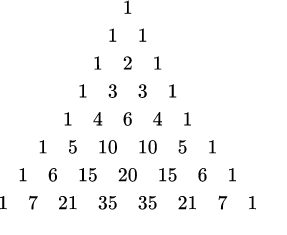
\includegraphics[width=\linewidth]{triangolo_di_tartaglia.png}
  	\caption{Triangolo di Tartaglia}
        \label{fig:triangolo_di_tartaglia.png}
\end{figure}


\end{document}
